\chapter{Contribuição}\label{meto}

A contribuição dessa pesquisa é de cunho metodológico-prático.
Do ponto de vista metodológico pela aplicação do processo CRISP-DM, usado para construir o modelo preditivo; do ponto de vista prático 
pela proposição de um modelo que integre predição à API de mapas de posicionamento global, fornecendo informação suficiente a um gestor para decidir quando 
e por onde enviar uma frota de caminhões por determinada rodovia que apresente retenções crescentes de logística de cargas. 

As soluções disponíveis que existem tais como; Google Maps, Waze e outros dessa natureza somente exibem informações momentâneas, produzidas e compartilhadas pelos utilizadores 
dos aplicativos ou por informações provindas de GPS, contudo não analisam dados históricos dessas rodovias nem fazem predições sobre o seu comportamento.

Outra contribuição dessa pesquisa é a proposição de um arco cibernético construído com a API de redes sociais.
Os ``feeds'' de notícias das redes sociais como o Twitter permitem analisar o contexto das rodovias com defasagem temporal muito pequena.
Os utilizadores dessas redes sociais contribuem com muita informação relevante como por exemplo o anúncio de uma paralisação que ocorrerá 
daqui a uma semana, a PRF de Pernambuco é outro contribuidor permanente; com seu canal no Twitter: @PRF191PE fornece diariamente informação das rodovias 
além de dados estatísticos. 

A monitoração de redes sociais é feita por Mineração de dados em textos, em que são verificas palavras chaves tais como: protestos, acidentes, paralisação, no caso
específico do nosso estudo.

Uma vez capturadas e tratadas, as informações desses ``feeds'' são direcionadas a um banco de dados. 
Foi escolhido o Sistema Gerenciador de Banco de Dados (SGBD) MySQL para tratar esses ``feeds'' do Twitter. 
A opção pelo MySQL foi devido às características que consideramos essenciais, tais como: licença para livre utilização, boa capacidade para gerenciar grande quantidade de 
dados e por seguir o padrão SQL-ANSI; portanto não foi necessário estudo mais aprofundado para operacionalizar; ``select'', ``insert'' e ``update''.


\section{Modelo Proposto}

A metodologia utilizada nessa pesquisa contempla um plano em três etapas, cada uma dividida em fases atinentes.
A primeira etapa da nossa metodologia completa o ciclo todo do processo CRISP-DM, onde está o modelo preditivo e 
a descoberta de conhecimento sobre o comportamento das rodovias estudadas. O descoberta de conhecimento sobre esses comportamento 
nas rodovias tem a ver com o ``modus operandi'' dos utilizadores, sobre possíveis erros de traçados e outros que possam
ser identificados pelos algoritmos de mineração empregados no processo.

A priori foram escolhidos algoritmos com algumas características especiais, tais como; robustez, tolerância à faltas (missing data),
taxa de aprendizagem, e facilidade de interpretação dos dados processados. 
No quesito robustez, tolerância à faltas e taxa de aprendizagem as redes neurais artificiais (RNA), com uma 
topologia Perceptron multicamadas com retroalimentação ``backpropagation'', essas redes destacam-se pela capacidade de generalização e 
especificidade em modelos de previsão. 

A extrapolação do modelo preditivo ocorre quando este se integra à uma estrutura dinâmica a serem exibidas em mapas vetoriais, 
dado um espaço temporal pré-determinado por um agente; o utilizador. 
Através de APIs os mapas vetoriais permitem a geolocalização dos pontos classificados ou os pontos onde haverá grande número de 
retenções, conhecido no meio da logística de cargas como \textbf{gargalo}.
A API do Google-Maps é o ``front end'', foi escolhida por permitir maior pela portabilidade e simplicidade para integração da estrutura
dinâmica com a preditiva.

Para a integração às redes sociais, foi escolhida a API do Twitter. Esta ``interface'' é simples de ser configurada e gera poucos dados; 
o utilizador tem que ser eficaz ao publicar suas postagem em um espaço de 140 caracteres, isso facilita a forma como os dados são
extraídos pela quantidade diminuta deles, bem como a quantidade conexões à Internet, contudo está rede social tem uma crescente quantidade
de postagens no formato imagens, isso dificulta a mineração em textos.
A API do Twitter tem a finalidade de integrar o modelo dinâmica dos mapas vetoriais às redes sociais. 
Esta ``interface'' é responsável por fornecer ``input'' à terceira etapa, servindo de ``busca local'' das informações mais recentes das 
redes sociais, relativas à trechos das rodovias; os ``feeds'' do Twitter (ou twetts) fornecem dados que serão minerados e interpretados à posteriori.

A figura a seguir ilustra (um overview) essa metodologia descrita graficamente.

\pagebreak

\begin{figure}[ht]
\centering
\caption{Etapas da modelo proposto}
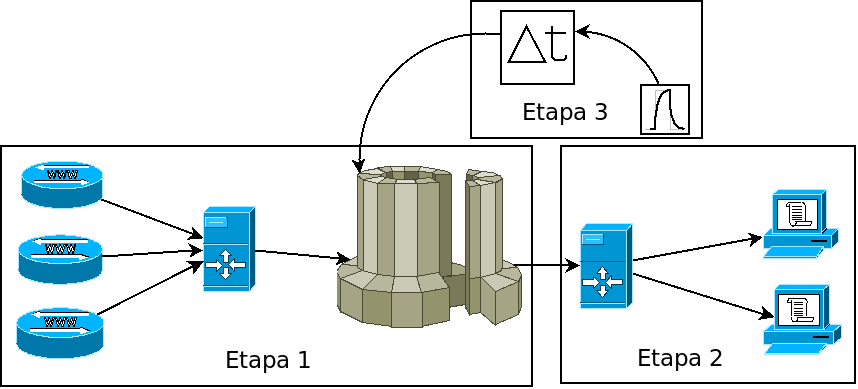
\includegraphics[width=170mm, height=85mm]{Figuras/Metodologia/metodologiaGeral.png}\\
\tiny Fonte: autor
\end{figure}

\section{Reflexão sobre as tecnologias utilizadas no modelo preditivo}\label{result}

Não existe uma técnica de mineração que generalize os mais diversos ambientes preditivos, mas sim um ``pool'' 
dessas técnicas onde uma complementa outra como identificamos nos artigos de ZENG, HUANG, PEI \textit{et al} (2016), 
POSSAS, BAV e CARVALHO (1998), e BESHAS e HILL (2010).

As técnicas preditivas tradicionais que contemplam análise de grandes massas de dados como base homogêneas.

são possíveis quando adaptadas para uma forma comparável à que
foram inicialmente concebidas, por que as variáveis em uma base de dados a priori guardam pouca relação as variáveis de outra base de dados.
neste caso essas variáveis ou são excluídas ou são transformadas a fim de ``guardarem'' um correlação com a outra base de dados. 

Na fase de transformação de dados, da primeira etapa, onde são criadas novas variáveis, a proximidade entre as
bases heterogêneas foi conseguido utilizando de regras de indução da lógica proposicional \cite{NorvigRussel2004}.
Nesta pesquisa, bases heterogêneas foram integralizadas num única grande conjunto de dados o ``data set''. As variáveis desse ``data set''
são consideradas variáveis independentes, foram preservadas as com maior relevância ou as que continham a maior quantidade de conhecimento
embutido.  construídas novas, nas bases onde não haviam correspondência, respeitando a lógica do negócio.\\
A tabela a seguir descreve as variáveis originais na base de dados de acidentes da PRF 

\pagebreak

\section{Extração do conhecimento - KDD}

O processo de descoberta do conhecimento iniciou-se com a coleta das bases de dados de acidentes da PRF. Optamos por coletar os dados dessa base diretamente na fonte,
ou seja dos servidores da PRF. Esses dados nos foram cedidos após alguns procedimento burocráticos de praxe (ver anexos). Essa escolha foi motivada para tentar
mitigar o problema da qualidade dos dados. No artigo ``Uma análise da qualidade dos dados relativos aos boletins de ocorrências das rodovias 
federais para o processo de Mineração de Dados'' COSTA, BERNARDINI, LIMA et al (2012) destacam a não padronização e não aceitação dos dados pela 
comunidade internacional. EAVES, D. (2009) sugere que os dados sejam disponibilizados na maneira como foram coletados.

A PRF tem ao menos duas bases \footnote{Somente mencionamos bases de dados que foram interessantes à essa pesquisa.} de dados referentes às ocorrências 
nas rodovias BRs. A base de acidentes rodoviários e a base de intervenções que ``guarda as ocorrências que paralisaram as rodovias, tais como:
protestos ou paralisações dessa natureza, feitos pelas pessoas que vivem no entorno dessas rodovias.

As técnicas como Redes Neurais Artificias (MLP) \cite{DecisaoCredito}, Árvores de decisão (CART) \cite{DataMining}, Regressão logística (MLR) 
\cite{RegrecaoLog} fornecem visão generalizada dos fatores preponderantes, levantando padrões ocultos nos dados. Esta fase é conhecida como 
Aprendizagem de Máquina (acrônimo de Machine Learning)

\begin{itemize}
 \item[a] Redes Neurais Artificias do tipo \textit{ Multi Layer Perceptron}  -- (MLP) têm capacidade de receber várias entradas ao mesmo tempo e distribuí-las de maneira organizada, além 
	  são simples de implementar e trazem resultados satisfatórios em grandes bases de dados.
 
 \item[b] Árvores de decisão do tipo \textit{ Classification and Regression Tree}  -- (CART) foi empregue por Pakgohar et al no artigo 
	  \textit{The role of human factor in incident and severity of road crashes based on the CART and LR regression a data mining approach}  para classificar acidentes 
	  com nível de acurácia próximo aos 80\%

 \item[c] Regressão logística tipo \textit{Multinomial Logistic Regression} -- (MLR) fornece a possibilidade de aprofundamento em vários níveis de busca sendo a mais apropriada, já que Regressão logística 
	  tradicional não permite aprofundamento desse tipo no espaço de busca.
\end{itemize}


\section{Extrapolação para georreferenciamento}

\pagebreak

\section{Arco cibernético com dados do Twitter}

Os dados do Twitter, permite uma busca imediata por novas informações que poderão ser confrontadas com o 
modelo preditivo aumentando o nível de confiança deste, com isso a informação construirá um Arco cibernético, que segundo Wiener (1948) a 
informação permite realimentação aos sistemas, com controle mais eficaz, por exemplo: no trecho da Br 101, na altura do km 5, no 
Município de Goiana alguém publicou que a comunidade que mora no entorno dessa localidade fará um protesto daqui a dois dias devido ao 
acidente ocorrido ou a PRF publicou que o km 80 da Br 232, na altura do Município de Gravatá será interditada amanhã, por 2h, para 
remoção/explosão de rochas. 
Essas informações, por serem a posteriori às predições, podem aumentar o nível de confiança sugerida pelo modelo preditivo e controle por 
parte do utilizador e dentro de um universo temporal mais restrito servir de comprovação do das predições.

No entanto pode ocorrer o contrário quando as informações provenientes do modelo de predição entrar em conflito com as informações 
provenientes das redes sociais \footnote{O sistema de predição é baseado em cálculos probabilísticos}, para estes casos a decisão de 
qual ação a ser tomada sempre estará ``nas mãos'' do agente, o observador ou o utilizador.

As informações das redes sociais, armazenadas em um banco de dados, poderão servir futuramente para novas predições.
Essas informações que comporão o arco cibernético não deverão retroalimentar o modelo de predição já construído, pois o fluxo decisório
já foi tomado pelo observador, sendo que dados a posteriori não servem para um modelo de predição, enviesa o sistema preditivo.
Uma nova fase de Mineração de Dados, desta vez mineração de dados em textos com modelo de predição. 
Dessa forma compõe-se um novo arco cibernético, mais genérico à proposição inicial descrita.

\begin{figure}[ht]
\centering
\caption{O arco cibernético com o Twitter}
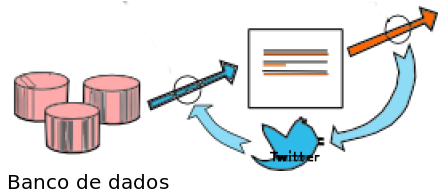
\includegraphics[width=90mm, height=45mm]{Figuras/Metodologia/ArcoCibernetico.png}\\
\tiny Fonte: autor
\end{figure}




